\documentclass{article} % \documentclass{} is the first command in any LaTeX code.  It is used to define what kind of document 

\usepackage{amsmath} % \usepackage is a command that allows you to add functionality to your LaTeX code            
\usepackage{mathtools}
\usepackage{graphicx}

\title{Math215} % Sets article title

\author{Homework 6, Problem 2} % Sets authors name
\date{\today} 

\begin{document} % All begin commands must be paired with an end command somewhere                    
\maketitle % creates title using infromation in preamble (title, author, date)
\section*{11.1 Problem 12} % creates a section
Find and sketch the domain of the function: $f(x,y,z) = ln(16 - 4x^2 - 4y^2 - z^2)$
\\\\Solution:
\begin{equation*}
  16 - 4x^2 - 4y^2 - z^2 > 0
\end{equation*}
\begin{equation*}
  4x^2 + 4y^2 + z^2 < 16
\end{equation*}
\begin{equation*}
  \frac{x^2}{4} + \frac{y^2}{4} + \frac{z^2}{16} < 1
\end{equation*}
\begin{equation*}
  \frac{x^2}{2^2} + \frac{y^2}{2^2} + \frac{z^2}{4^2} < 1
\end{equation*}
\\The domain is an ellipsoid bounded by $\frac{x^2}{2^2} + \frac{y^2}{2^2} + \frac{z^2}{4^2} < 1$
\\ 
\\
\begin{center}
  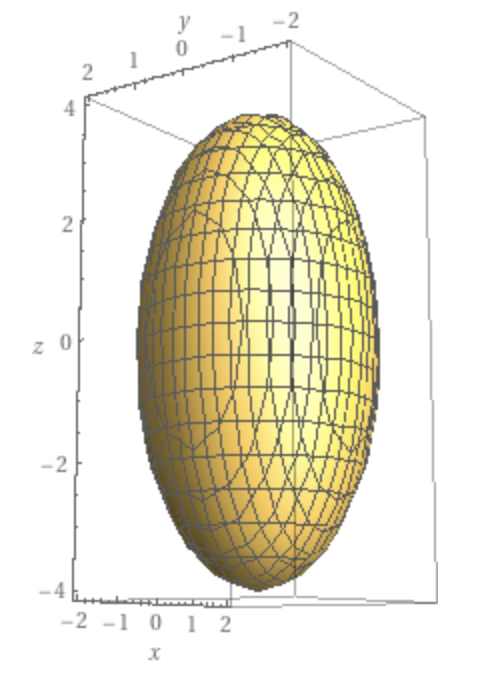
\includegraphics[height=3in]{graph.png}
\end{center}
  
\end{document}
